The aLIGO interferometers are highly complex, high precision devices. 
Their operation depends on the careful interaction of a series of subsystems, 
each with its own purpose. In an effort to better understand the operation 
and output of the interferometers, the Detector Characterization group has 
been designed to mirror this subsystem approach. Table 
\ref{table:aligo-subsystems} lists the aLIGO subsystems. Each of these 
subsystems is assigned a data quality liaison from the DetChar group. 

\begin{table}[ht!]%
  \begin{center}
    \begin{tabular}{|c|l|}
    \hline
    Subsystem & Description \\
    \hline
    LSC & Length Sensing and Control \\
    \hline
    ASC & Alignment Sensing and Control \\
    \hline 
    SUS & Suspensions \\
    \hline
    IMC & Input Mode Cleaner \\
    \hline 
    OMC & Output Mode Cleaner \\
    \hline
    PCAL & Photometric Calibration \\
    \hline 
    PEM & Physical Environmental Monitoring \\
    \hline
    SEI & Seismic Isolation \\
    \hline
    PSL & Pre-Stabilized Laser \\
    \hline
    TCS & Thermal Compensation System \\
    \hline
    \end{tabular}
  \end{center}
  \caption[Table of aLIGO subsytems]{Table describing aLIGO subsystems}
  \label{table:aligo-subsystems}
\end{table}

There are 5 main responsibilities assigned to a subsystem liaison. The 
first is to fully understand the operation and installation of the subsystem 
so that they can faciliate data quality investigations and act as a 
point of contact for commissioners assigned to this subsystem.

The second responsibility 
is to take this knowledge and use it to populate the channel information 
system (CIS), which is a database that stores information about how to 
parse and understand the various auxiliary channels that are monitored 
in each subsystem. This database also contains information about calibration 
and valid frequency ranges for these channels. This allows newcomers to the 
collaboration to more easily familiarize themselves with the LIGO naming 
conventions and facilitates their involvement in data quality investigations.  

The third responsibility 
is to check for signal fidelity, which means to make sure that all of the 
channels are working as intended and don't contain artifacts from signal 
conditioning processes.

The fourth responsibility is to develop summary pages that monitor 
important channels and figures of merit for each subsystem. 
The summary pages are generated 
every day from a configuration file designed by the subsystem liaisons. 
The purpose of the summary pages is to gather all of the potentially 
useful information about a subsystem in an organized way so that the 
subsystem leads can efficiently evaluate the performance of the subsystem. 
They are also a useful launch point for data quality 
investigations since they provide various overviews of instrumental 
performance ($h(t)$ spectrograms, Omicron triggers, CBC search sensitivity, etc.) 
that make it easy to identify persistent or egregious data quality issues.

The fifth and final responsibility is to develop and build real-time 
data quality monitors in the Online Detector Characterization (ODC) 
framework. 
The Online Detector Characterization (ODC) system is an infrastructure designed
to extract and record metadata describing the state of the aLIGO interferometers.
This state information has two main purposes: to inform data quality investigations
and to serve as a real-time monitor of the interferometer state
that can be accessed in the control room. Each subsystem is monitored 
using an ODC monitor.

The ODC system is unique in that it is runs in real-time in the 
system that is used to control the LIGO interferometers. Each set of ODC monitors
is built in Simulink to directly interface with the models that control the 
interferometers. This has several distinct advantages.
Since the monitors are run in real-time, they operate in parallel with the control
loops that are sensing the various degrees of freedom of the interferometer and are
able to achieve highly precise timing. The ODC monitors can also create their own
test points, which means an ODC monitor can perform a check on any signal that exists
in the front end at its full rate instead of relying on the information that is
downsampled and stored on disk.
These full rate test points operate at the full sample rate of the model (16384 Hz)
and any information recorded in the ODC channel is written at the same rate. In contrast,
many channels are only recorded at 16 Hz if they aren't accessed as a test point in the digital 
system.

The information generated by each ODC monitor can be extracted and sent to a segment
generation process, where the most useful information is catalogued and represented by
segments of time that indicate when a given condition was considered to be true or false.

\section{Length Sensing and Control}

The Length Sensing and Control (LSC) subsystem is 
used to monitor and control the lengths of the various optical cavities in the 
aLIGO interferometers. Figure \ref{fig:aligo-simple} shows the layout 
of the aLIGO interferometer with the lengths of individual optical cavities 
labeled. 
The LSC subsystem is responsible for controlling 5 global degrees of freedom, 
which are linear combinations of these individual cavity lengths. Table 
\ref{table:aligo-dofs}  
describes the degrees of freedom controlled by the LSC subsystem. 
The most important degree of freedom in the LIGO interferometers is the Differential 
Arm length (DARM), which is the degree of freedom that is sensitive to the differential 
stretching and squeezing of spacetime caused by a gravitational wave. The Common Arm length 
(CARM) is the average arm length of the two interferometers. This degree of freedom is 
imporant for ensuring that both arms are held at their resonance length and is used to 
counteract effects such as slow drift from tidal forces. The Michelson (MICH) degree of 
freedom measures the differental arm length of the small Michelson interferometer formed 
by the two ITMs and the beamsplitter. This is an important degree of freedom because 
noise in this degree of freedom will result in excess light at the readout port of the 
interferometer. The final two degrees of freedom are the Power Recycling Cavity Length 
(PRCL) and the Signal Recycling Cavity length (SRCL). These are resonant cavities formed 
between the recycling mirrors and the ITMs. PRCL must be controlled to maintain a steady 
level of optical power in the interferometer, as modulating this length will modulate 
the power recycling gain in the interferometer. The signal recycling cavity forms a coupled 
cavity with the arms and must be controlled to maintain the 
frequency response of the interferometer. 

\begin{figure}
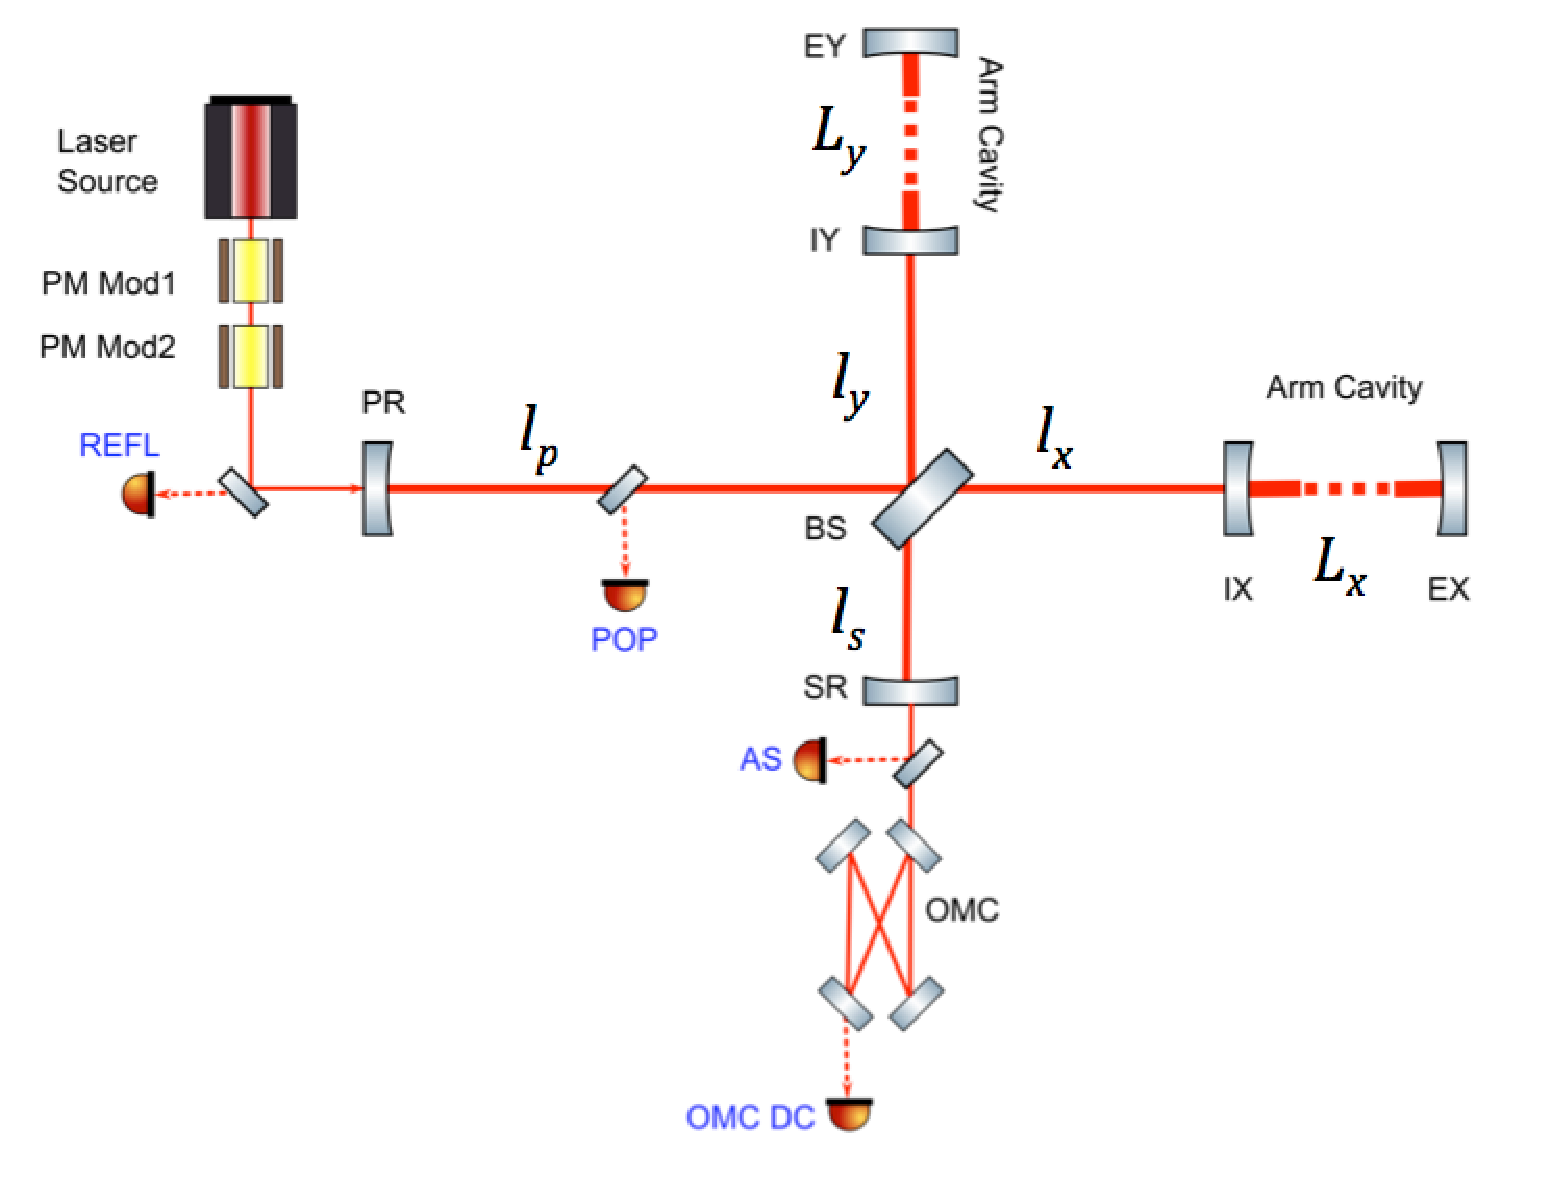
\includegraphics[width=\textwidth]{figures/ODC/aligo-simple}
\caption[LIGO length degrees of freedom]{A simplified layout of a LIGO interferometer %
         with the lengths of optical cavities labeled. These optical cavities combine %
         to form 5 global degrees of freedom that are controlled by the Length Sensing %
         and Control subsystem. Reproduced from \cite{Kokeyama:detchar}.}
\label{fig:aligo-simple}
\end{figure}

\begin{table}[ht!]%
  \begin{center}
    \begin{tabular}{|c|c|}
    \hline
    Degree of Freedom & Description \\
    \hline
    Differential Arm (DARM) & $L_x - L_y$ \\
    \hline
    Common Arm (CARM) & $(L_x + L_y)/2$ \\
    \hline 
    Michelson (MICH) & $l_x - l_y$ \\
    \hline
    Power Recycling Cavity Length (PRCL) & $l_p + (l_x + l_y)/2$ \\
    \hline 
    Signal Recycling Cavity Length (SRCL) & $l_s + (l_x + l_y)/2$ \\
    \hline
    \end{tabular}
  \end{center}
  \caption[Table of LIGO degrees of freedom]{Table of LIGO length degrees of freedom}
  \label{table:aligo-dofs}
\end{table}

Length Sensing and Control is a critical subsystem that is used to control
not only the auxiliary optical cavities, but the DARM degree of freedom which
is sensitive to gravitational wave signals.
These optical cavities are controlled using the Pound-Drever-Hall (PDH) 
technique described in Chapter \ref{ch:IMCUpconversion}.

\subsection{Online Detector Characterization}

The ODC model for the LSC subsystem is designed to monitor the feedback 
loops used to control optical cavities. A series of test points are placed 
in the control loop and compared to user-set threshold values to determine 
whether or not they are in their nominal range. 
Figure \ref{fig:lsc-odc-model} shows the implementation of an LSC ODC 
model in SIMULINK. The numbered ovals on the left of the image are test point 
signals that are being read in from the higher level model that is used to control the 
lengths of the optical cavities. The signals are carried along the wires connecting 
each box. The green boxes are where the user set thresholds are saved. The white 
boxes perform operations on input signals.

As an example, we'll follow the path of inputs 46 and 47, which are signals from 
the photodiode that measures the reflected light at the input to the power recycling 
cavity. The signals are read in at the ovals labelled 46 and 47, their absolute values 
are calculated at the boxes labeled 'Abs19' and 'Abs20'. The absolute values of these 
signals are then fed into boolean comparison boxes, 'Operator39' and 'Operator40'. 
These boolean operator boxes are also connected to the green box which defines a 
threshold for the signals to be compared to. If the input signals are less than the 
designated threshold, the boolean operator passes a value of True. If they have 
exceeded the intended threshold, the boolean operator passes a value of False. 
The outputs of the two boolean operators are fed into one last check, which performs 
an AND operation. If both signals have passed their tests and reported True, the AND 
block reports a True and this photodiode signal is considered to be in a good state. 
If one or both of the signals has failed their test, the AND block reports a False 
and the photodiode signal is considered to be in a bad state. 

Some of the checks implemented in the ODC models are more complicated. For 
example, when 
the states of multiple control loops are stored in a vector they can be compared to a 
series of state masks that select which degrees of freedom to check. 
In this way, the same vector of information used to perform hierarchical 
checks on the state of the instrument. 
One test can check that the core optics are performing nominally, a more broad 
test can include checks on both the core optics and recycling cavities, and 
then the overall test can be done to check that feedback loops are performing as intended. 
Each of these tests will report its own true or false answer. 

\begin{figure}[ht!]
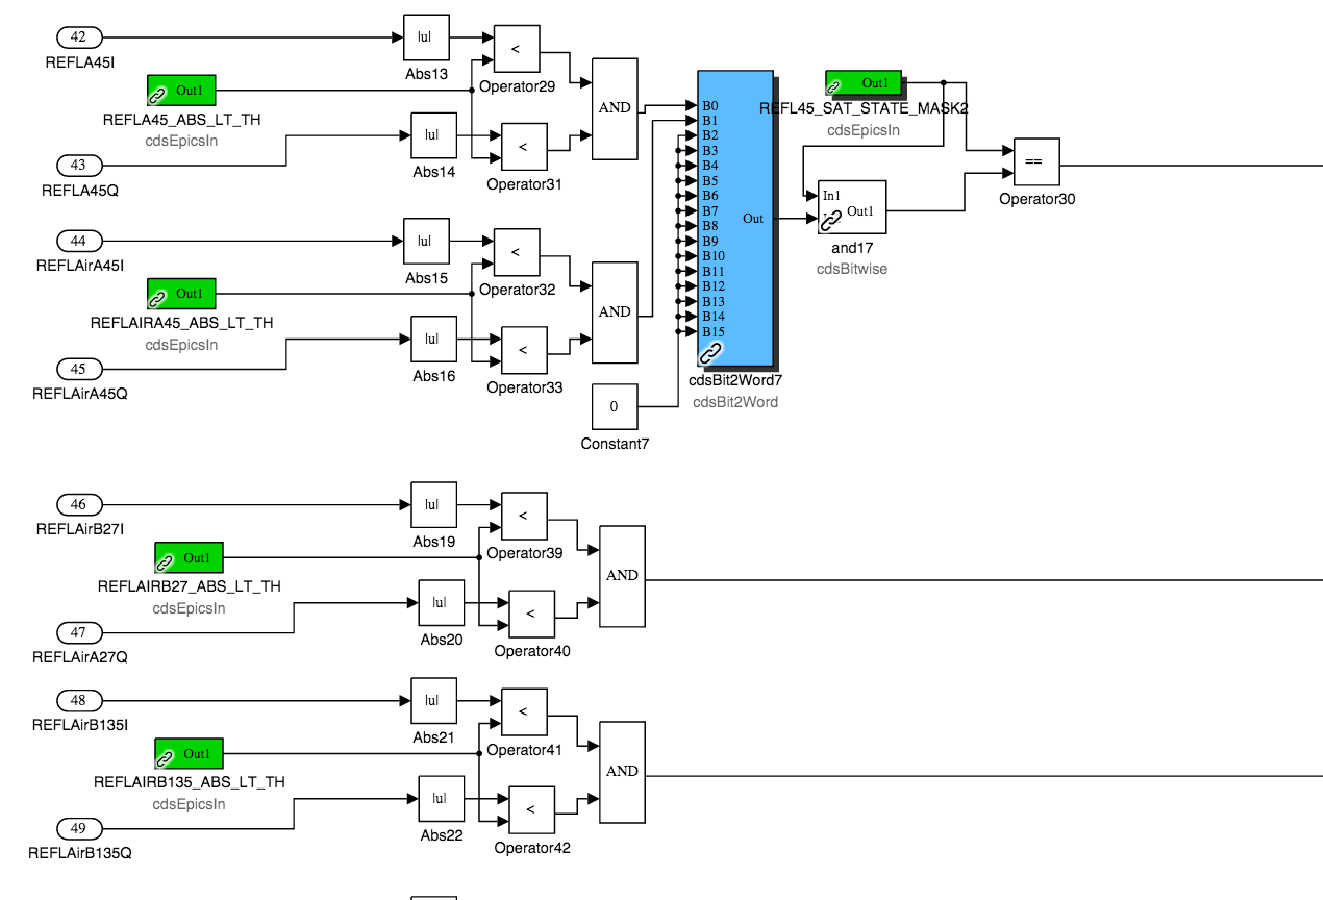
\includegraphics[width=\textwidth]{figures/ODC/LSC-ODC-model}
\caption[LSC ODC SIMULINK Model Example]{LSC ODC checks implemented in SIMULINK. %
         The numbered ovals on the left indicate signals used in real-time control %
         of the interferometer. The green boxes represent user-defined threshold %
         values to be used in boolean comparisons. The white boxes represent operations %
         such as computing the absolute value of a signal or performing boolean %
         comparisons (less than, greater than, AND, OR, etc.)}
\end{figure}\label{fig:lsc-odc-model}

Once the ODC model has performed all of its checks and reported a True or False 
answer, the information is stored in an overall state vector that can be parsed to 
learn the state of the LSC subsystem at any time. 
Figure \ref{fig:lsc-odc-bits} shows a visual representation of the state of the 
length degrees of freedom in the H1 interferometer over the course of a day.
Each horizontal bar represents the state of a length degree of freedom as 
reported by ODC. In this particular day, the control signals for the Michelson 
(MICH) and signal recycling cavity (SRCL) degrees of freedom exceeded their 
nominal range while the interferometer was in its nominal operating state. 
This is indicated by the color of the bars switching between 6:00 - 8:00 UTC 
and between 14:00 - 16:00 UTC. All of the times when the state changes are 
recorded as time segments which can be used to correlate excursions in the 
cavity control signals with transients in the output of the interferometer. 

\begin{figure}[ht!]
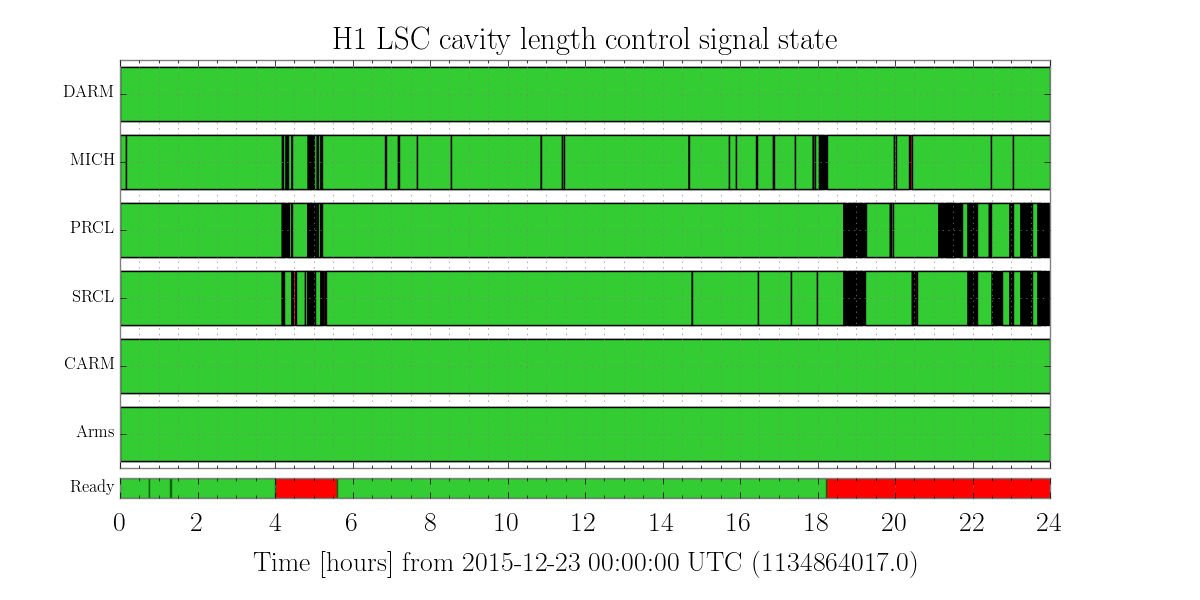
\includegraphics[width=\textwidth]{figures/ODC/LSC-bit-example}
\caption[LSC ODC bits example]{ODC bits representing states of length degrees of %
         freedom. Each horizontal bar represents a length degree of freedom that %
         is controlled in the LSC subsystem. When the bar is green, the control %
         signal for that degree of freedom is in its nominal range. When the %
         bar is not green, the control signal for that particular length degree %
         of freedom has exceeded the threshold set in the ODC model and is reported %
         as out of range.}
\label{fig:lsc-odc-bits}
\end{figure}

\subsection{MEDM screens}

For real-time use of these monitors, a software package called MEDM is used to 
display and interact with the ODC models. MEDM can be used to update the thresholds 
and state masks used to determine the status of a given photodiode or degree of 
freedom. 
Figure \ref{fig:lsc-odc} shows the LSC ODC overview screen in MEDM. 
The top panel summarizes the overall state of the subsystem, showing the state of 
each ODC bit and a bitmask that indicates whether or not a given bit is used in 
determining the overall state of the subsystem. 
The leftmost 
panel is used to monitor the state of each length degree of freedom in the interferometer. 
The rest of the panels are used to monitor the states of the various photodiodes used 
for sensing length degrees of freedom. These include DC power monitors and the values 
of RF demodulated photodiode signals. The grey boxes containing numerical values indicate 
user-set thresholds that can be updated from this screen.

\begin{figure}[ht!]
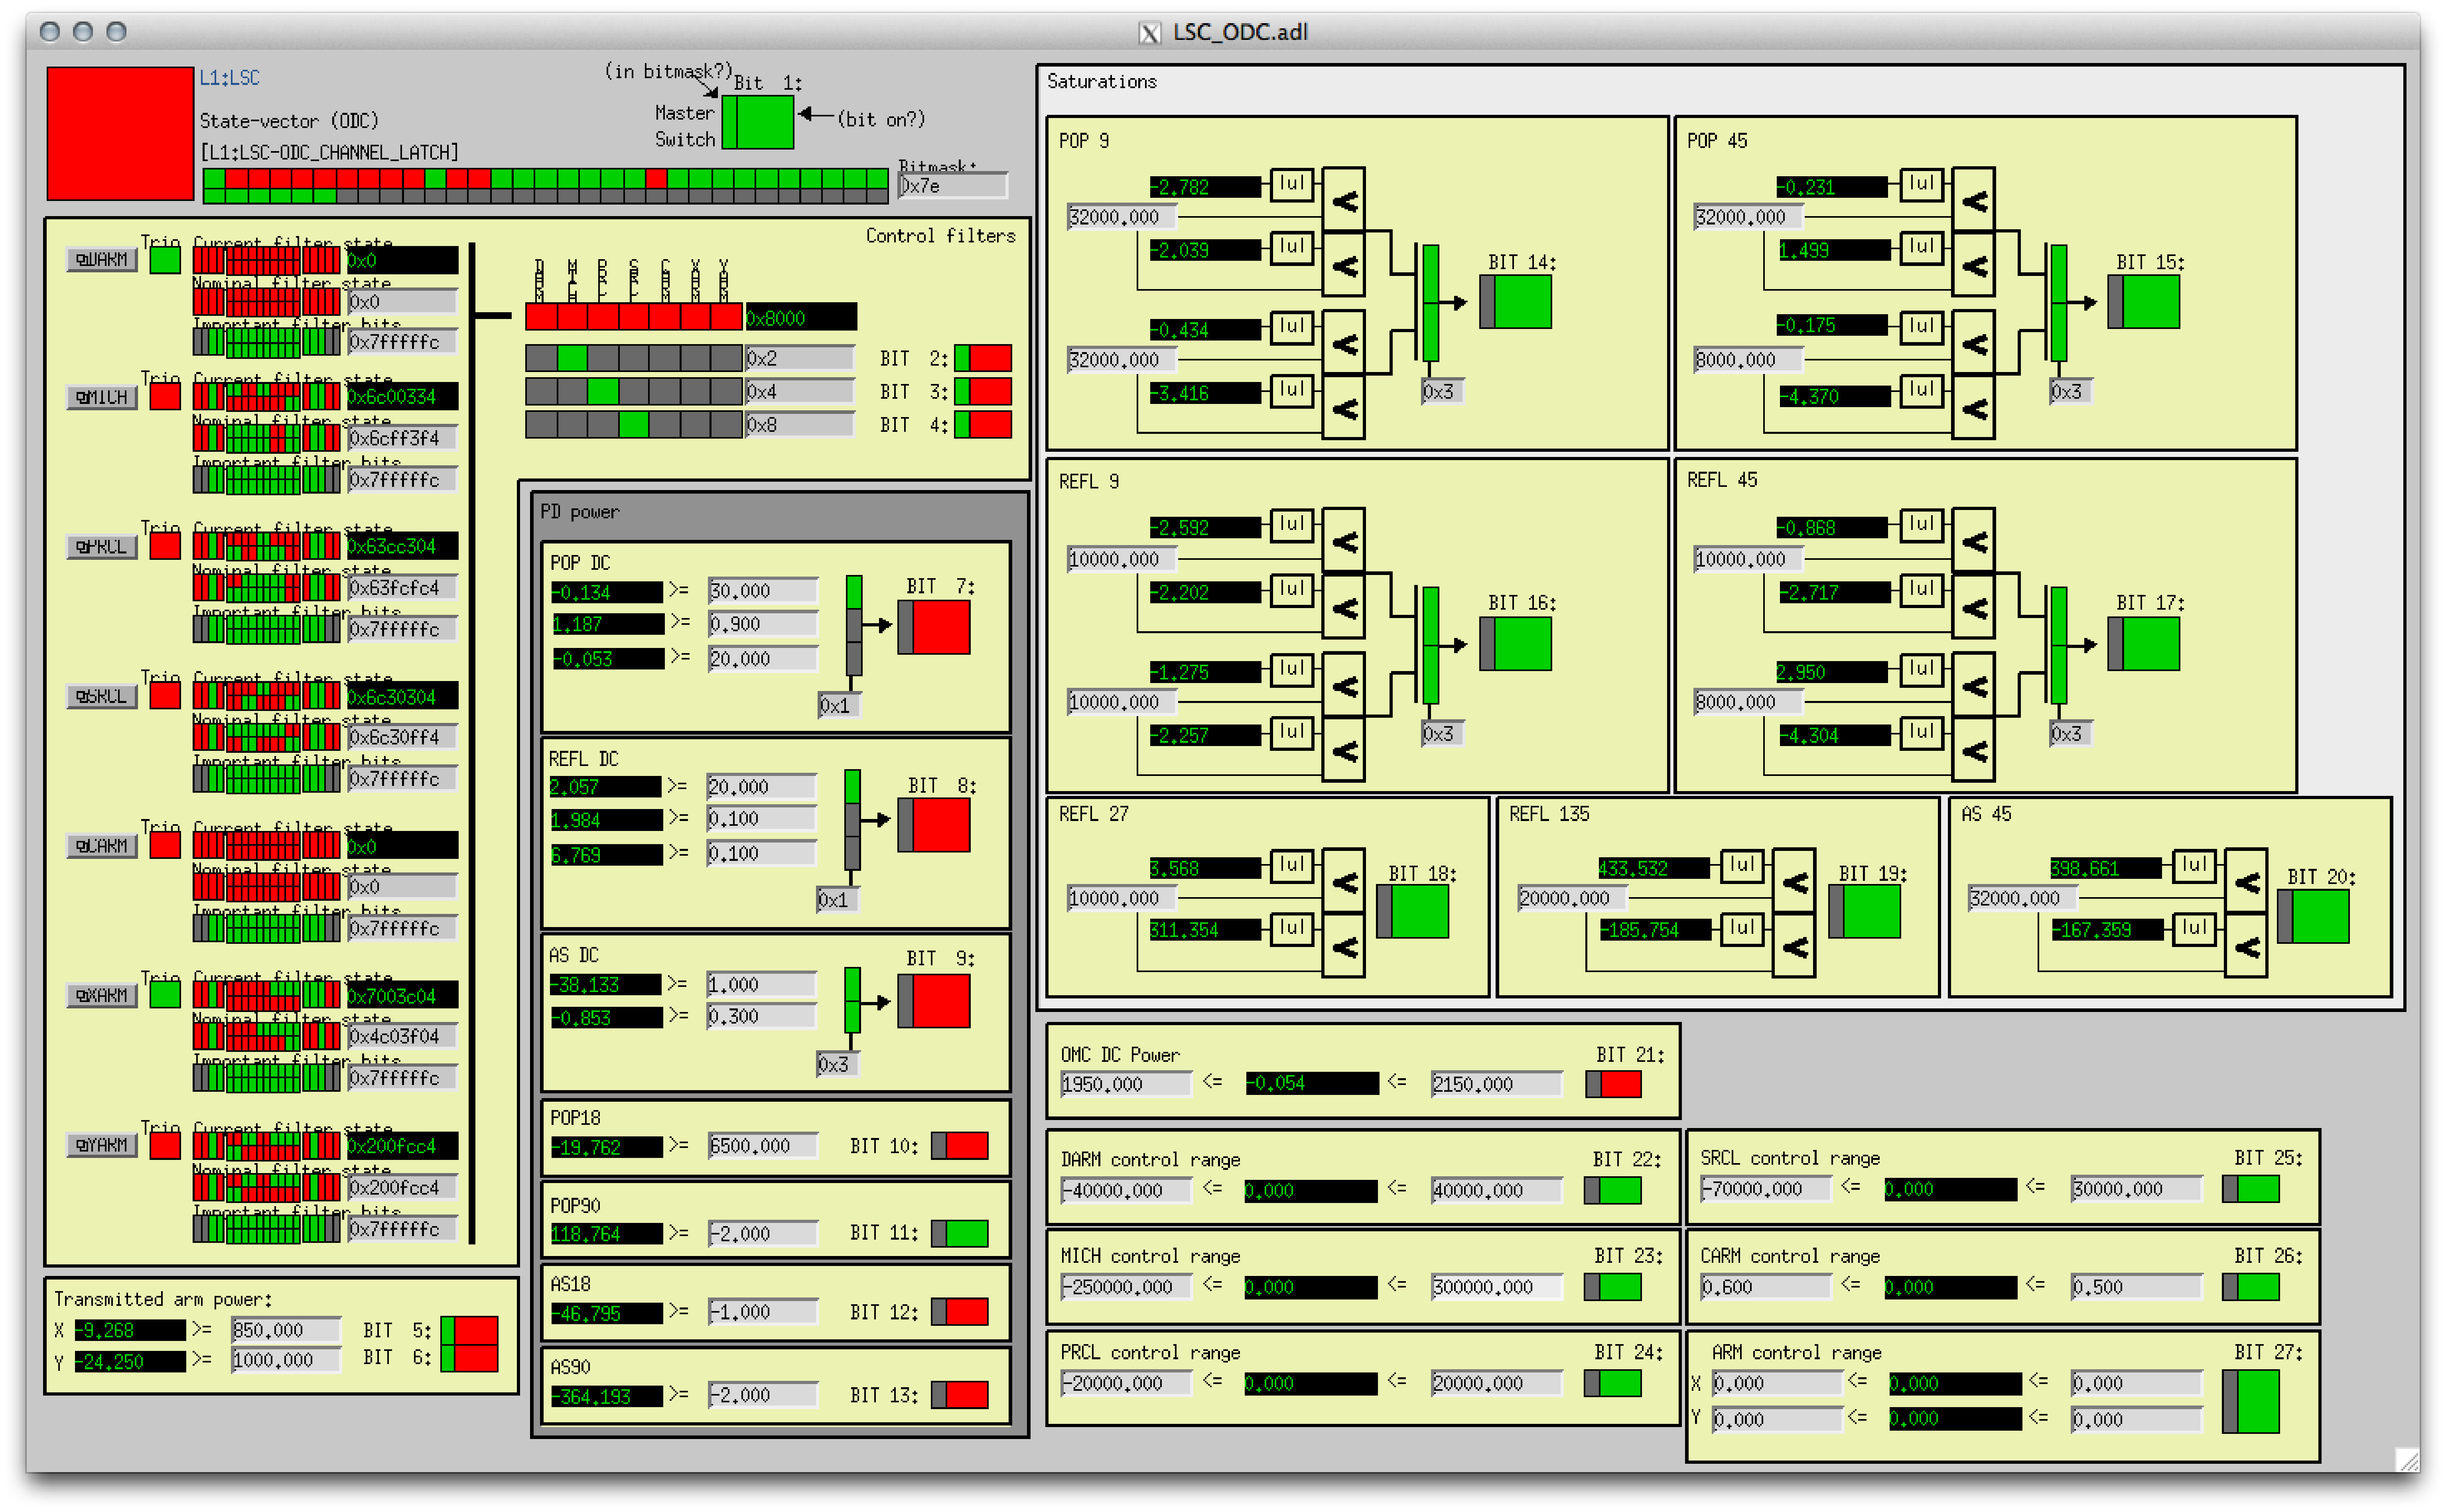
\includegraphics[width=\textwidth]{figures/ODC/LSC_screen}
\caption[LSC ODC Overview Screen]{MEDM screen used to interact with the LSC ODC model. %
         This screen contains information regarding the overall state of the LSC subsystem, %
         the state of control loops pertaining to specific length degrees of freedom in the %
         interferometer, and the state of photodiodes used to sense length degrees of freedom %
         in the interferometer.}
\label{fig:lsc-odc}
\end{figure}

\subsection{Summary pages}

While the MEDM screens are useful for real-time readout of the ODC models, they do not 
have an easily accessible history. For this reason, summary pages were built that 
contain the most important information from each ODC model. The summary pages are 
built multiple times per day and are accessible through a web browser, which allows 
easy, organized access to past interferometer data when performing a data 
quality investigation. 

Figure \ref{fig:lsc-odc-bits}, which shows the status of the length degrees of freedom 
of the interferomter over the course of a day, was taken from the summary pages. In this 
figure, the MICH degree of freedom was seen to move into a bad state during a locked state. 
As an example, we can look at the summary page visualization of the MICH degree of freedom 
during this time. 
Figure \ref{fig:mich-summary-pages} shows the control signal for the MICH degree of freedom 
with the ODC threshold 
overlaid as a dashed red line. The solid blue line indicates the median value of this signal 
over the course of 1 minute and the shaded regions indiate the maximum and minimum values over 
this same stretch of time. When the control signal exceeds the ODC threshold, such as at 
about 14:35 UTC, the corresponding bit in Figure \ref{fig:lsc-odc-bits} flashes red to 
indicate the excess noise in this channel. 

\begin{figure}[ht!]
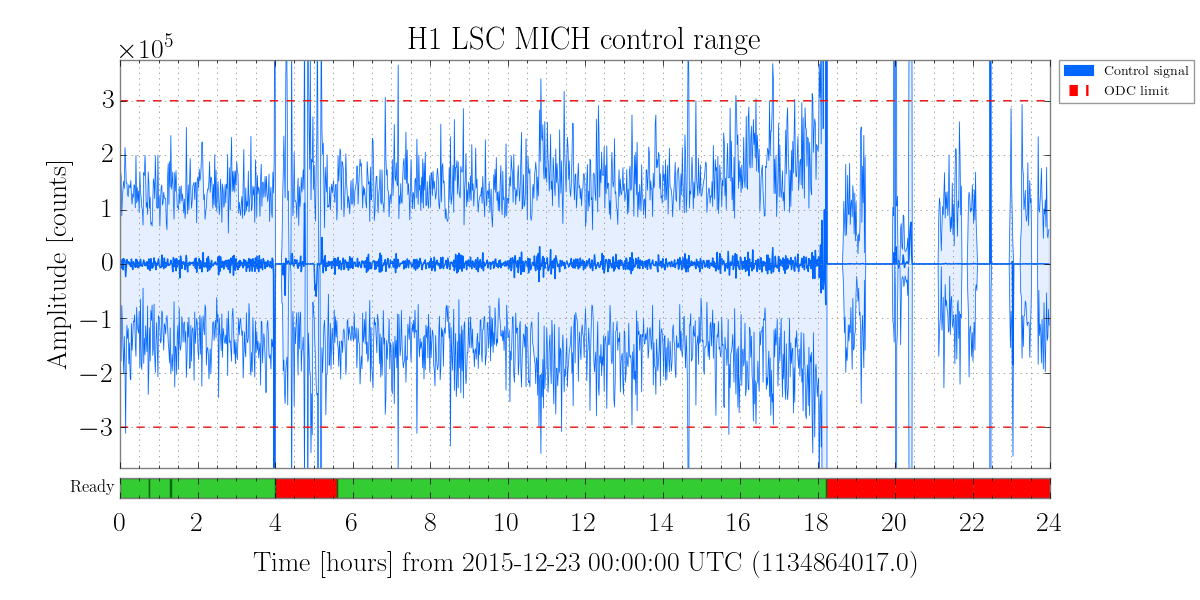
\includegraphics[width=\textwidth]{figures/ODC/H1-MICH-SUMMARY-PAGES}
\caption[MICH control signal on summary pages]{Readout of the MICH degree of freedom as %
         displayed on the summary pages. The dark blue curve indicates the median value of %
         the MICH control signal over the course of 1 minute. The shaded regions indicate %
         the maximum and minimum values of the control signal over the same stretch of time. %
         The dashed red line indicates the ODC threshold set to monitor this control signal.}
\label{fig:mich-summary-pages}
\end{figure}

\section{Alignment Sensing and Control}

The alignment sensing and control subsystem is used to control the alignment of 
optical cavities as well as the input pointing of light into those cavities. 
The control loops work in a similar way to the length sensing and control subsystem, 
using the reflected light from optical cavities to control the optics in a PDH 
scheme. The same set of RF sidebands that are used for length control are also used 
for alignment control. The detail that allows length fluctuations to be decoupled from 
alignment fluctuations is that alignment fluctuations generate higher order 
modes in the optical field, which are used to 
generate an error signal.

A length control loop compares the TEM00 mode of the carrier beam to the TEM00 
mode of the RF sidebands. 
An alignment control loop will compare the TEM00 mode of the carrier 
beam with the TEM10 and TEM01 modes of its sidebands, which are generated by 
angular misalignments of optical cavities. 
Since each optic has two alignment degrees of freedom that are directly 
controlled, pitch and yaw, and each cavity is comprised of multiple optics, 
the reflected light from each cavity is read out on a 
pair of quadrant photodiodes. This is visualized in Figure \ref{fig:odc-pd-screen}. 
The four quadrants allow the pitch and yaw error 
signals to be decoupled. Since higher order optical modes have a different Gouy 
phase as they propagate through space, a pair of photodiodes separated by a Gouy 
phase telescope are used to determine the origin of the misalignment 
\cite{NergisThesis}.

\subsection{Online Detector Characterization}

Given that the alignment sensing control subsystem is designed similarly 
to the length sensing and control subsystem, the general layout of the ODC 
model is very similar. The photodiodes signals used to generate alignment 
error signals are checked against a saturation threshold. The control 
signals that are sent to the optics are checked to ensure that they aren't 
exceeding their nominal range. Each degree of freedom is represented as one 
bit in a state vector, which can be compared to a series of state masks to 
check for a series of valid states. 

\subsection{MEDM screens}

The MEDM screens for the ASC subsystem are similar to those built to monitor 
the LSC subsystem. 
Figure \ref{fig:asc-odc} shows the ASC ODC overview screen in MEDM. 
The top panel once again describes the overall state of the subsystem and 
shows which ODC bits are used to determine that state. The left panel shows 
the status of the control signals used for each of the alignment degrees of 
freedom in both pitch and yaw. The bottom right panel, labeled 'QPD Saturations', 
checks for saturations in each of the quadrant photodiodes used in the ASC subsystem. 
Since there are many more checks that need to be made for the quadrant photodiodes, 
each one has a dedicated subscreen.

\begin{figure}[ht!]
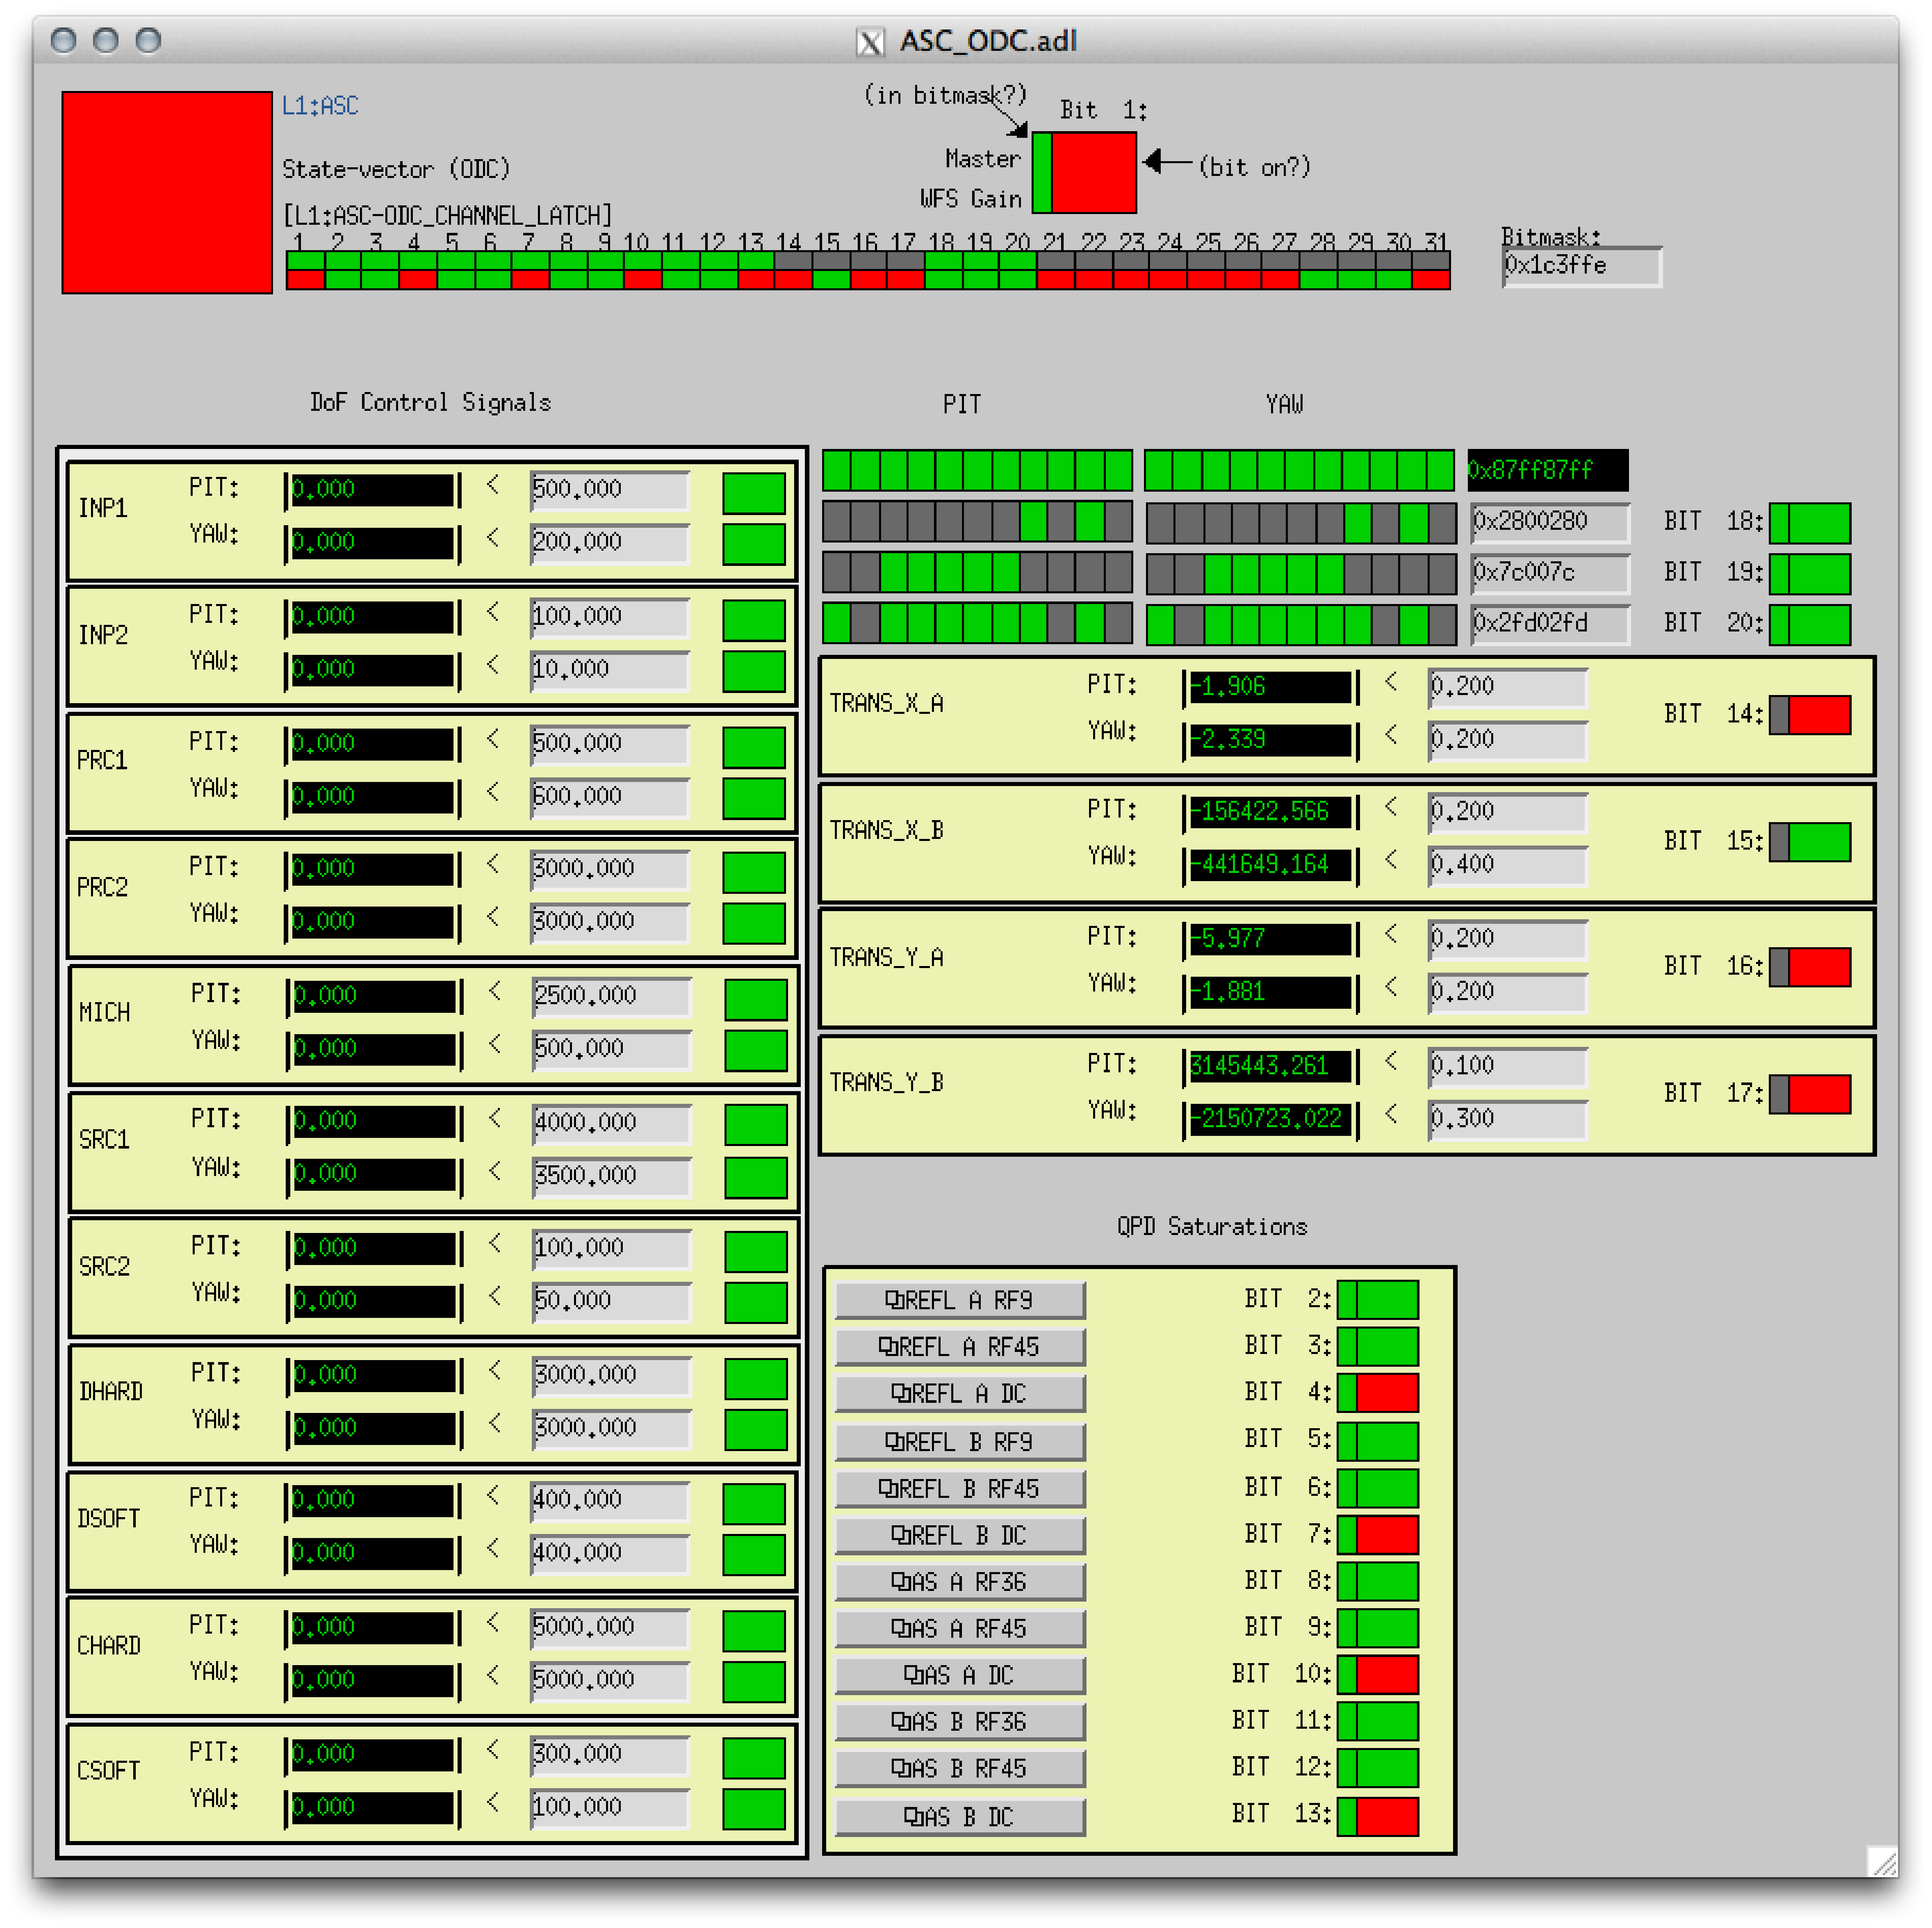
\includegraphics[width=\textwidth]{figures/ODC/ASC_screen}
\caption[ASC ODC Overview Screen]{MEDM screen used to interact with the ASC ODC model. %
         This screen shows the overall state of the ASC subsystem, the state of each %
         alignment degree of freedom in the interferometer, and the state of each %
         quadrant photodiode used to sense misalignments in the interferometer.}
\label{fig:asc-odc}
\end{figure}

Since the ASC subsystem uses quadrant photodiodes, each quadrant must be checked 
for saturation. 
Figure \ref{fig:odc-pd-screen} shows a photodiode monitor screen in the ASC ODC. 
The first and second panels show the readouts of each quadrant of a quadrant 
photodiode in I- and Q-phase respectively. The absolute value of each signal is 
calculated and compared to a threshold value to see if any quadrants are approaching 
a saturation limit. The third and fourth panels perform checks on the associated 
pitch and yaw readouts from these photodiodes to check for excursions beyond the 
nominal threshold. The nominal values for the pitch and yaw degrees of freedom 
are determined by trending these values over long durations of good interferometer 
performance.

\begin{figure}[ht!]
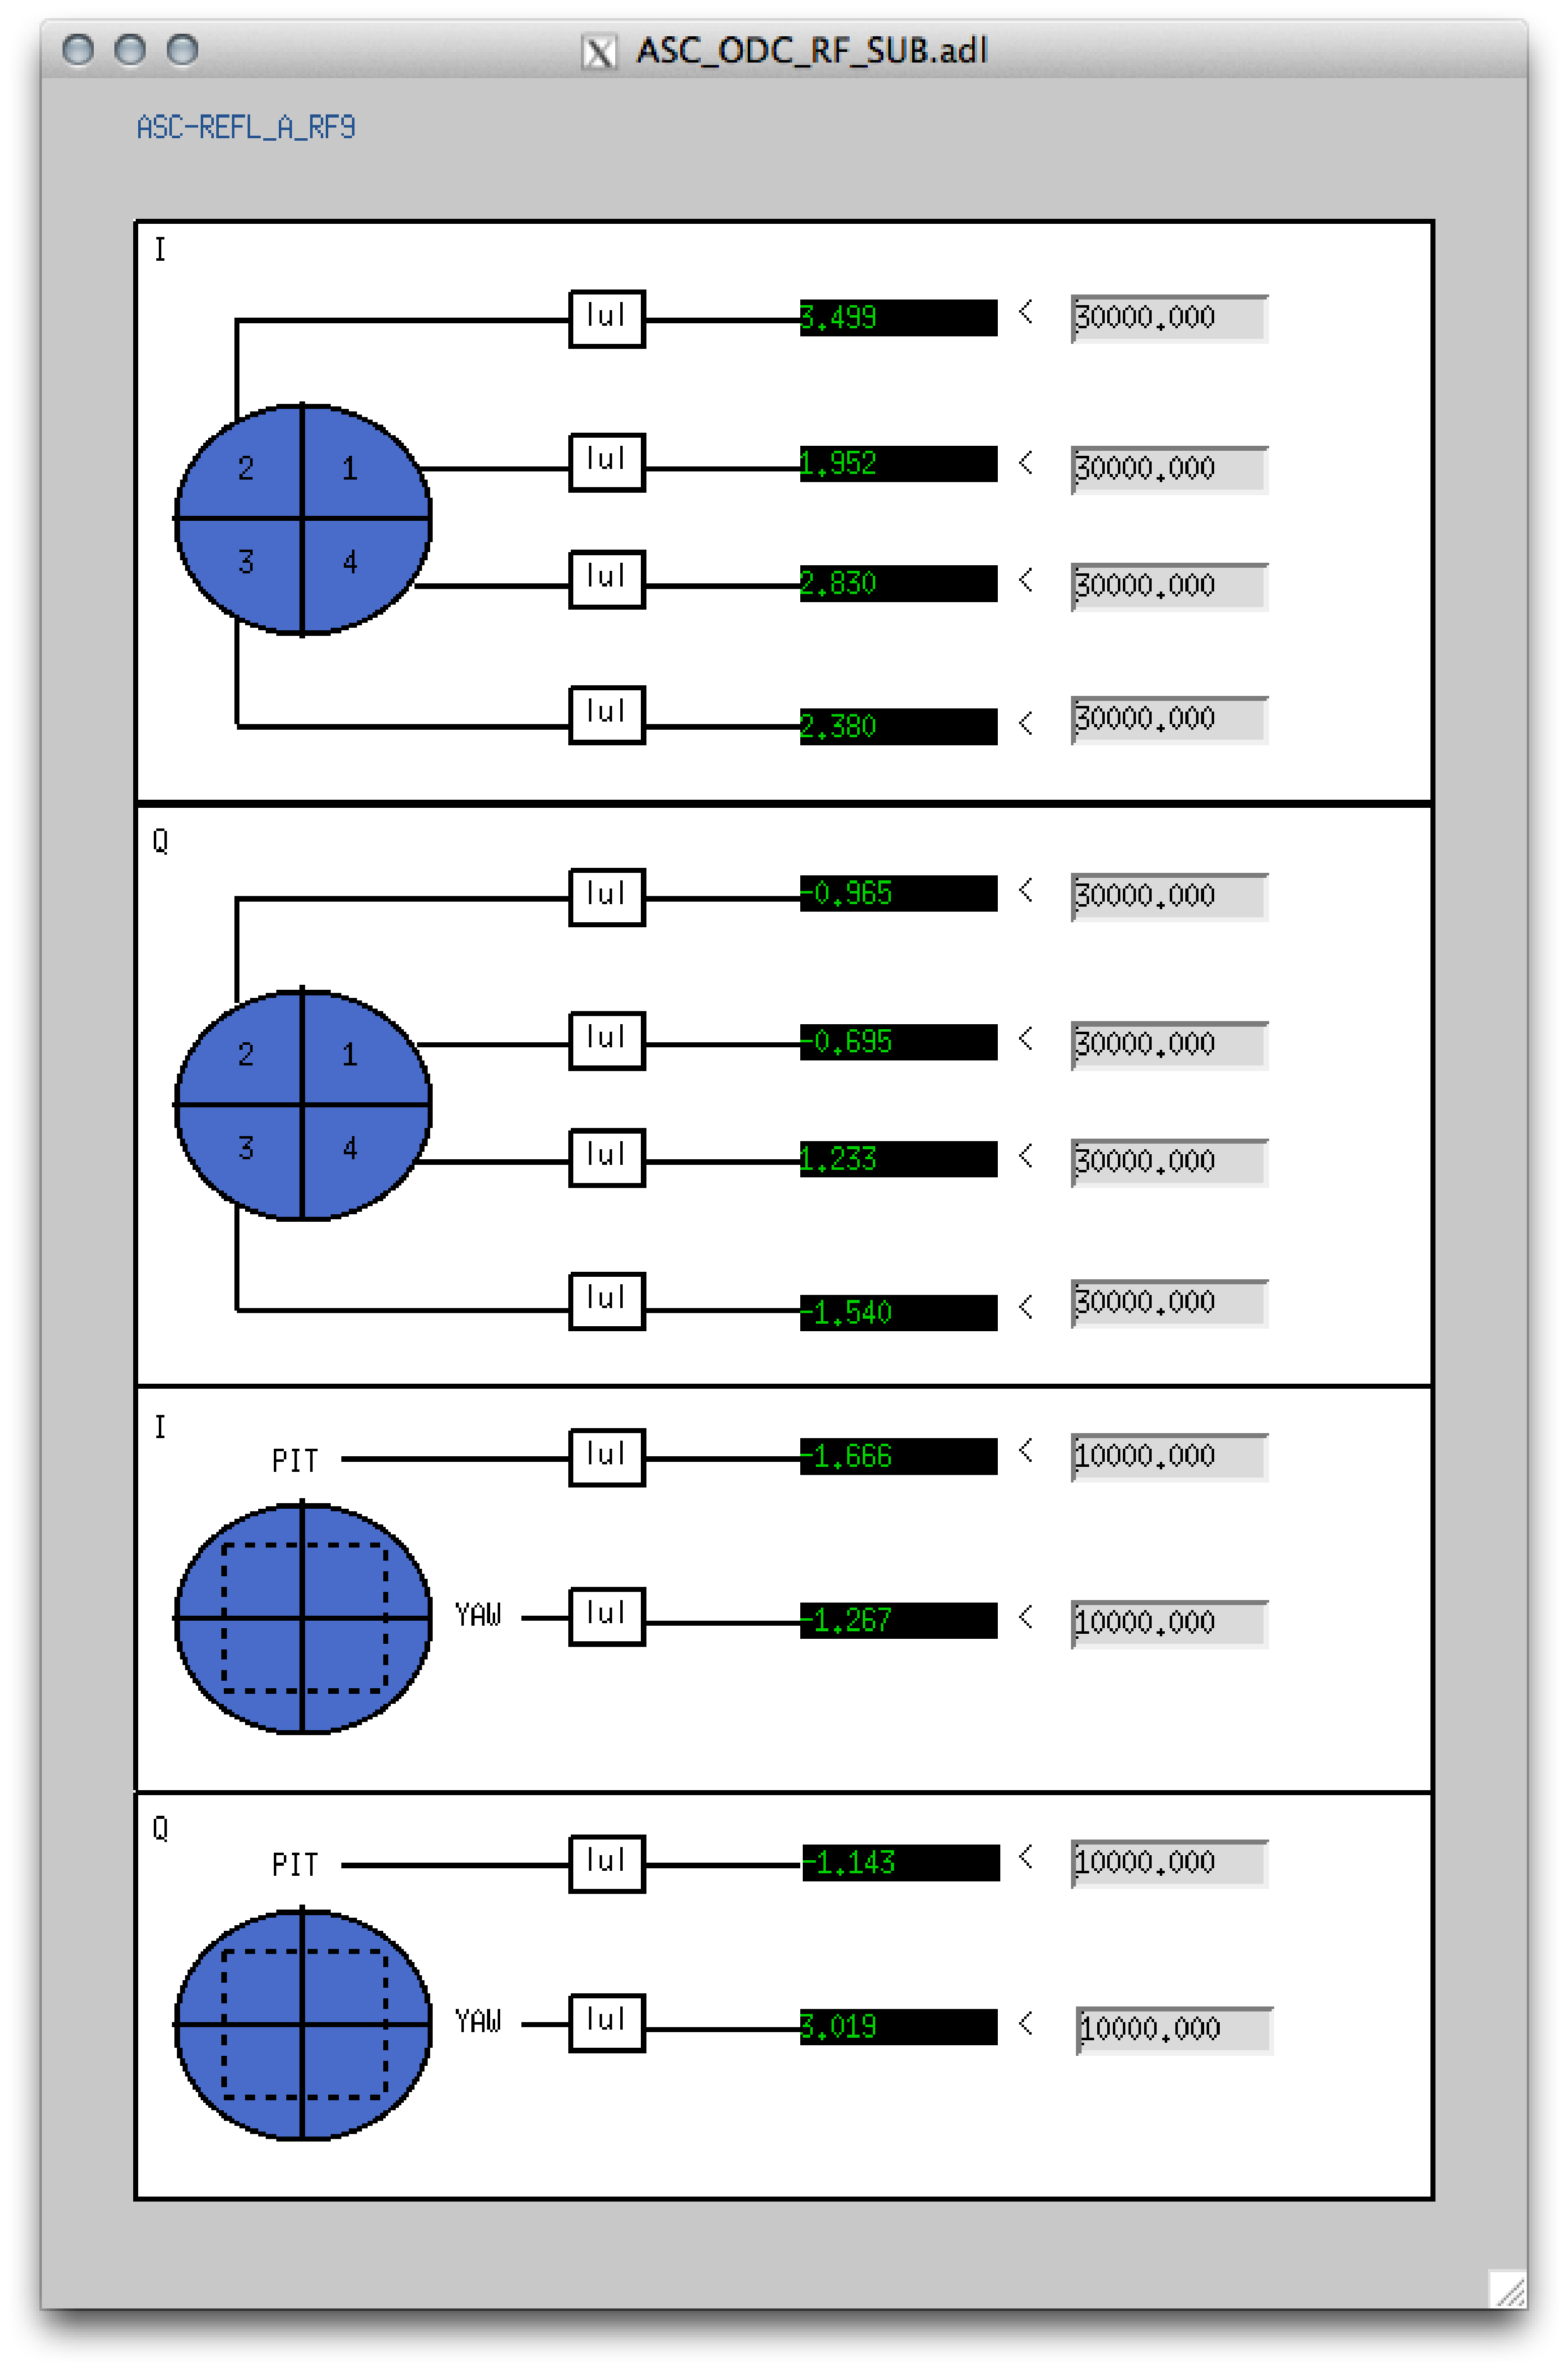
\includegraphics[width=0.7\textwidth]{figures/ODC/PD_screen}
\caption[ASC ODC Photodiode Monitor in MEDM]{ODC monitor for ASC photodiode in MEDM}
\label{fig:odc-pd-screen}
\end{figure}

\subsection{Summary pages}

The ASC subsystem also has an accompanying set of summary pages that keep a running 
record of its state. These summary pages are designed similarly to the LSC summary 
pages, including time-series of the control signals for each alignment degree of freedom, 
saturation monitors for the ASC photodiodes,  
and ODC plots indicating the state of each degree of freedom.

\section{ODC Results}

The ODC system was designed and implemented in the engineering runs that preceded the 
first observing run. During the first observing run, the first efforts were made to 
use the information reported by the ODC models to flag and understand noisy data. 
The most useful 
used the excess noise in the Michelson pitch degree of freedom to flag upstream 
electronics issues that caused loud glitches in $h(t)$. There is also evidence 
that the overall alignment status reported by the ASC ODC can be used as an early 
warning that the interferometer is going to drop out of its nominal operational 
state.

\subsection{MICH ODC as a witness of RF45 glitches}

The ODC channel built to monitor the Michelson (MICH) pitch degree of freedom 
was used to generate vetoes used in O1 analyses. Throughout O1, the H1 
interferometer was prone to a glitch mechanism driven by malfunctions in 
RF electronics used to generate frequency sidebands on the carrer beam. 
These RF sidebands are used to control auxiliary degrees of freedom in the 
interferometer, including the length of the small Michelson interferometer 
formed by the beamsplitter and the two ITMs. When the RF electronics glitched, 
the error signals of these cavities would also glitch, causing excess motion 
in the auxiliary degrees of freedom that was witnessed by ODC monitors set 
up to monitor the control signal of the MICH alignment control loops. 

Figure \ref{fig:mich-odc-example} 
shows the correlation between the witness channel for this ODC channel 
and glitches in $h(t)$ as identified by Omicron. Figure \ref{subfig:mich-odc-timeseries} 
shows a time-series the control signal of the MICH pitch control loop. The ODC threshold, 
set at a value of 250 for this particular channel, is indicated by the green dotted 
line. Any time the control signal crosses this threshold, a time segment is created to 
indicate that the control loop is not in a nominal operating state. Figure 
\ref{subfig:mich-odc-omicron} shows the $h(t)$ Omicron triggers over the same 
duration. When the MICH pitch control point has a high variance, for example 
in the first 1.5 hours of the plot, there is an 
overall increase in the rate of high SNR Omicron triggers, indicating that 
this ODC channel is witnessing alignment fluctuations that couple into the 
output of the interferometer. 

\begin{figure}[ht!]%
\subfloat[]{
  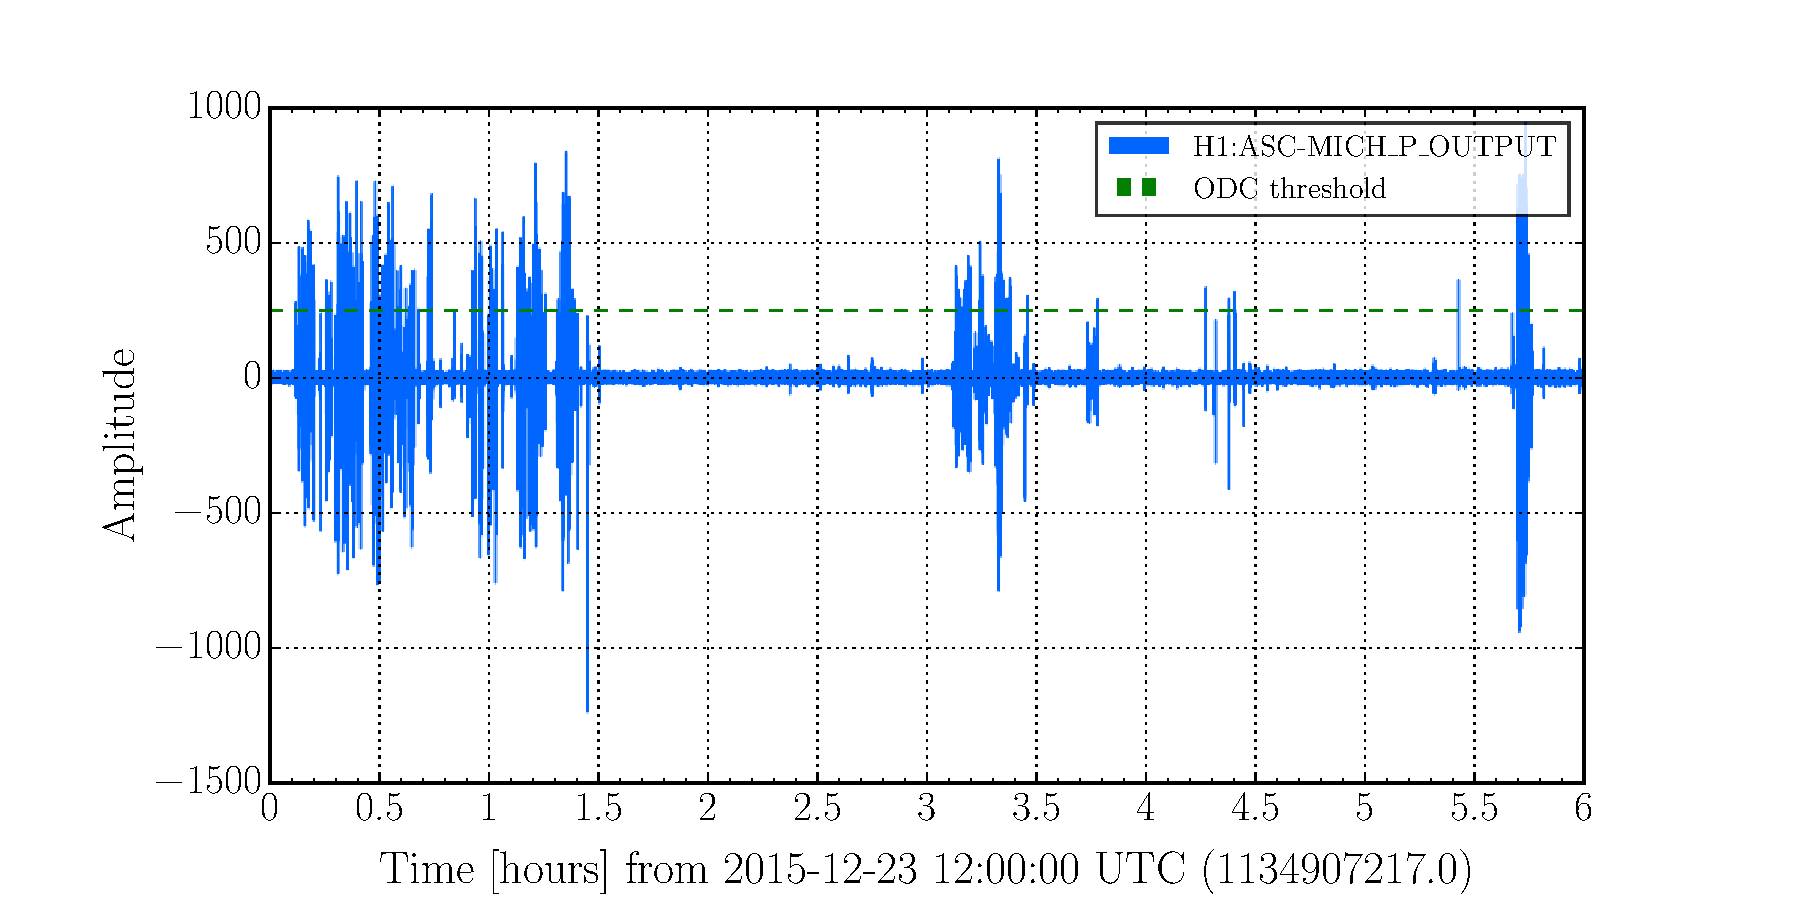
\includegraphics[width=\textwidth]{figures/detchar/MICH_P_OUTPUT_ODC}
  \label{subfig:mich-odc-timeseries}
  }

\subfloat[]{
  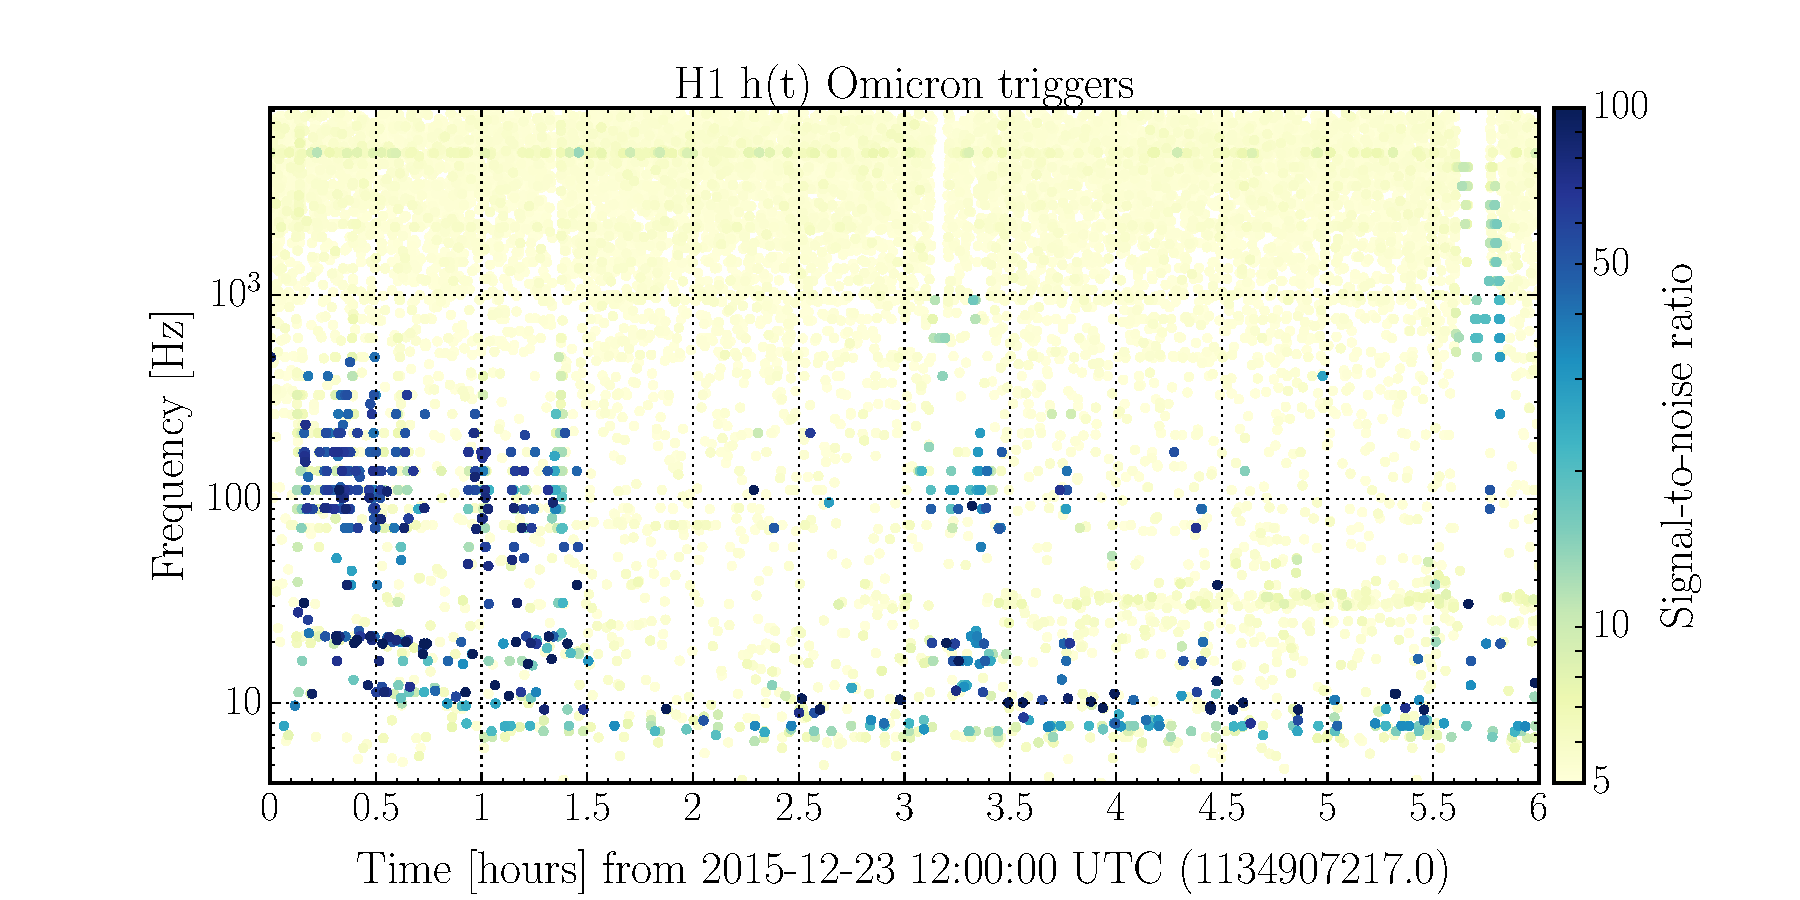
\includegraphics[width=\textwidth]{figures/detchar/Omicron_MICH_ODC}
  \label{subfig:mich-odc-omicron}
  }
\caption[ODC threshold on MICH pitch]{%
         An example of an ODC channel witnessing RF electronics issues, which %
         manifested as angular fluctuations in the vertex degrees of freedom %
         at H1. Figure \ref{subfig:mich-odc-timeseries} shows the ODC threshold %
         marking fluctuations in the MICH pitch degree of freedom. Figure %
         \ref{subfig:mich-odc-omicron} shows the associated Omicron triggers from %
         $h(t)$ at the same time. The storms of loud triggers between 10 - 400 Hz %
         are coincident with times flagged by this ODC monitor.}
\end{figure}\label{fig:mich-odc-example}

This coupling can be quantified by removing these times from the output of the 
interferometer and calculating how efficiently this removal of time captures 
transient noise in $h(t)$. The 
time segments generated by this ODC channel are very efficient at vetoing high SNR 
Omicron triggers. Removing these segments of time from $h(t)$ removes Omicron triggers 
with SNR $>$ 8 with an $\frac{efficiency}{deadtime}$ ratio of 47.16, indicating that 
a large number of high SNR Omicron triggers are removed from $h(t)$ while removing 
very little time from the analysis. These 
time segments, when used in the search, are called data quality vetoes. These vetoes 
were included were distributed to the CBC and Burst searches in O1 to indicate time 
that should not be analyzed. (Further discussion of data quality vetoes can be found 
in Chapter \ref{ch:Vetoes}.

